\subsection{Functional requirements}
\par
The functional requirements will be listed with different way:
\begin{itemize}
\item Some will be called core requirements, which is necessary to satisfy more or less every goals in a simple way (e.g. registration, log-in, ...)
\item Other requirements are listed together with the goal which they satisfy
\end{itemize}

\subsubsection{Core requirements}
\par
The following requirements are, principally, about identifying a specific person on the system:
\begin{itemize}
\item[{[R1]}] Allow a person to register into the system as a user by providing a username, a password, his credentials, his social security number and a consensus on the agreement
\item[{[R2]}] Allow a person or company to register into the system as a third party by providing an e-mail, a password, its credentials and a consensus on the agreement
\item[{[R3]}] A person cannot register as a user by inserting a username that has already been used in another successful registration process
\item[{[R4]}] A person cannot register as user by using the same social security number used in another successful registration process 
\item[{[R5]}] A person cannot register as user by using the same credential used in another successful registration process 
\item[{[R6]}] A person or company cannot register as third party into the system by using the same credentials used in another successful process
\item[{[R7]}] A person or company cannot register as third party by using the same e-mail used in another successful registration process
\end{itemize}
\par
After the registration, another essential functionality of the system is to permit log-in:
\begin{itemize}
\item[{[R8]}] Allow a person to log into the system as a user only if he has already registered as such
\item[{[R9]}] Allow a person or company to log into the system as a third party only if he has already registered as such
\end{itemize}

\subsubsection{Goal reaching requirements}
\par
In this section, each requirement is necessary to satisfy specific goals of the system:
\begin{itemize}
\item[{[G1]}] Allow a user to access its own data
	\begin{itemize}
	\item[{[R10]}] If a user is logged-in, he is able to view its own data
	\end{itemize}
\item[{[G2]}] Allow a user to contribute to data sharing by providing information about his location and health status
	\begin{itemize}
	\item[{[D1]}]  User's smartphones are equipped with GPS sensor
	\item[{[D2]}] Users own devices with sensors to acquire data information about health status
	\item[{[D3]}] Health data collected by the devices are correct
	\item[{[D6]}] There is at least an external service of trusted companies which provides the possibility to transfer data from devices containing sensors to acquire health data to smartphones
	\item[{[R11]}] Allow a user to send its data to the system automatically when it is generated
	\end{itemize}
\item[{[G3 \& G4]}] Once the health parameters of a user have been observed 
below the threshold for the first time after one hour, an ambulance is sent to the user location. 
The time experienced between the moment in which the health parameters of a subscribed user are observed below the threshold and the time in which the emergency point is contacted is equal or less than 5 seconds
	\begin{itemize}
	\item[{[D5]}] There is at least an external service of trusted companies which provides the possibility to make automated calls
	\item[{[D8]}] Hospitals always accepts new SOSCall regarding a person which has not yet received help.
	\item[{[D9]}] If SOSCall are accepted, then an ambulance is sent to the location mentioned by the call
	\item[{[D13]}] After receiving help from an ambulance, a person can't be discharged before an hour
	\item[{[R12]}] When a user's health parameters has been observed below the threshold, an SOSCall is requested within 5 seconds
	\item[{[R13]}] All the automated SOS call are performed with devices of users whose health parameters are observed below a certain threshold
	\item[{[R14]}] An SOSCall can be requested only every minute
	\item[{[R15]}] An SOSCall is blocked if a previous one has already been accepted within one hour
	\item[{[R16]}] An SOSCall is implemented as an automated call by using an external service
	\end{itemize}
\item[{[G5 \& G6]}] Allow a user to participate in a run managed by third parties, as an athlete, if all starting conditions are satisfied. Allow a user to unsubscribe from a run before the expiration date
	\begin{itemize}
	\item[{[D14]}] Every user enrolled in a run are able to participate in the run as athletes if all starting conditions are satisfied
	\item[{[R17]}] Allow a user to view a list of available runs, i.e. those that are still waiting to start 
	\item[{[R18]}] Allow a user to enroll in a run, after choosing it from the list, only before the expiration date by specifying his nickname
	\item[{[R19]}] Allow a user to unsubscribe from an enrolled run only before the expiration date
	\end{itemize}
\item[{[G7]}] Allow spectators (i.e. user) to see on real-time the "correct" positions of all athletes taking part in a run, with at most 15 meters of radius error
	\begin{itemize}
	\item[{[D4]}] There is at least an external service of trusted companies which provides the possibility to the user to view detailed maps
	\item[{[D11]}] When a user's phone GPS is set on high precision, then it provides the right position with at most a radius error ranged from 0 to 10 meters
	\item[{[D12]}] Athlete participating in a run are equipped with a device sharing GPS position set on high precision
	\item[{[R20]}] Every athlete participating on a run, only on this specific occasion, shares continuously (i.e. each ten seconds) its position through a device
	\item[{[R21]}] Allow a spectator to see on a map the real-time position of every athlete in a specific run
	\end{itemize}
\item[{[G8]}] The maximum time to accept an individual request from any third party is 30 days; after that, the request will expire
	\begin{itemize}
	\item[{[R22]}] Once the time elapsed from sending request is greater than 30 days, then the request will be deleted from the system
	\end{itemize}
\item[{[G9 \& G10]}] Allow a user to accept or refuse a request from third parties. Allow a user to block requests made by a specific third party
	\begin{itemize}
	\item[{[R23]}] Allow a user to receive individual requests about data sharing from third parties
	\item[{[R24]}] Allow a user to view a list of pending requests
	\item[{[R25]}] Allow a user to accept or refuse a request from the list of pending request
	\item[{[R26]}] Allow a user to block requests from a defined third party, after refusing it
	\end{itemize}	
\item[{[G11]}] In case it is impossible to start a run, the enrolled runners are notified
	\begin{itemize}
	\item[{[R27]}] If, after the expiration date, the number of participants is less than the minimum number defined by the organizer, then it is impossible to start the run.
	\item[{[R28]}] If the run cannot start due to minimum number of participants unsatisfied, then the enrolled runners are notified.
	\end{itemize}
\item[{[G12]}] Allow spectators and runners to see the leaderboard, when a run is completed
	\begin{itemize}
	\item[{[D15]}]All the organizers close a race that has not been canceled due to starting conditions
	\item[{[R29]}] Allow an organizer to close the run (when it is terminated)
	\item[{[R30]}] After a run is closed, show the leaderboard to the spectators and runners
	\end{itemize}
\item[{[G13]}] Allow organizers (i.e. third parties) to set up a run, by defining its name, its path, date, start time, expiration date, and the minimum number of participants
	\begin{itemize}
	\item[{[D4]}] There is at least an external service of trusted companies which provides the possibility to the user to view detailed maps
	\item[{[D10]}] The service which shows the map of the world offers only paths that are feasible.
	\item[{[R31]}] Allow a third party to see a map of the world with feasible paths
	\item[{[R32]}] Allow a third party to publish a race by providing an unique name, a feasible and a non-overlapping path (non-overlapping with other races of the same date), a date, a start time, a brief description, an expiration date for subscription and a minimum number of participants
	\end{itemize}
\item[{[G14]}] Allow a third party to access data specified in a request if the user accepts the request or if he accepted one or more requests from the same third party that provided access to the same data 
	\begin{itemize}
	\item[{[R33]}] If an individual request is accepted, then the third party who has made the request can access the data specified in the request
	\item[{[R34]}] For each piece of individual data accessible by a third part customer, exists an accepted request regarding it, performed by the same third party 
	\item[{[R35]}] Allow a user to accept or refuse request given by third parties
	\item[{[R36]}] Allow a third party to send individual requests to users by providing the user's social security number and a brief motivation
	\end{itemize}
\item[{[G15]}] Allow a third party to access statistical and anonymized data if and only if the number of individual involved is greater than 1000. This is satisfied as soon as the request is approved  
	\begin{itemize}
	\item[{[R37]}] A group request is accepted if the aggregated data specified in the request is accessible to the third party who performed the demand
	\item[{[R38]}] Group requests are accepted if and only if the number of user involved is greater than 1000
	\item[{[R39]}] Aggregated data is accessible to a third party if an accepted aggregated data that request that data exists
	\item[{[R40]}] Allow a third party to send group request to the system regarding data about many users
	\end{itemize}
\item[{[G16]}] Allow a third party to subscribe to non-existing data. They will have access to them, as soon as the data is generated. 
	\begin{itemize}
	\item[{[R41]}] Allow a third party to express a data request on future data
	\item[{[R42]}] A third party can have access to non-existing aggregated data regarding future information if and only if the number of people involved will be greater than 1000
	\end{itemize}
\end{itemize}

\subsubsection{Use Case}
Here follows the use case diagram: \\

\begin{figure}[H]
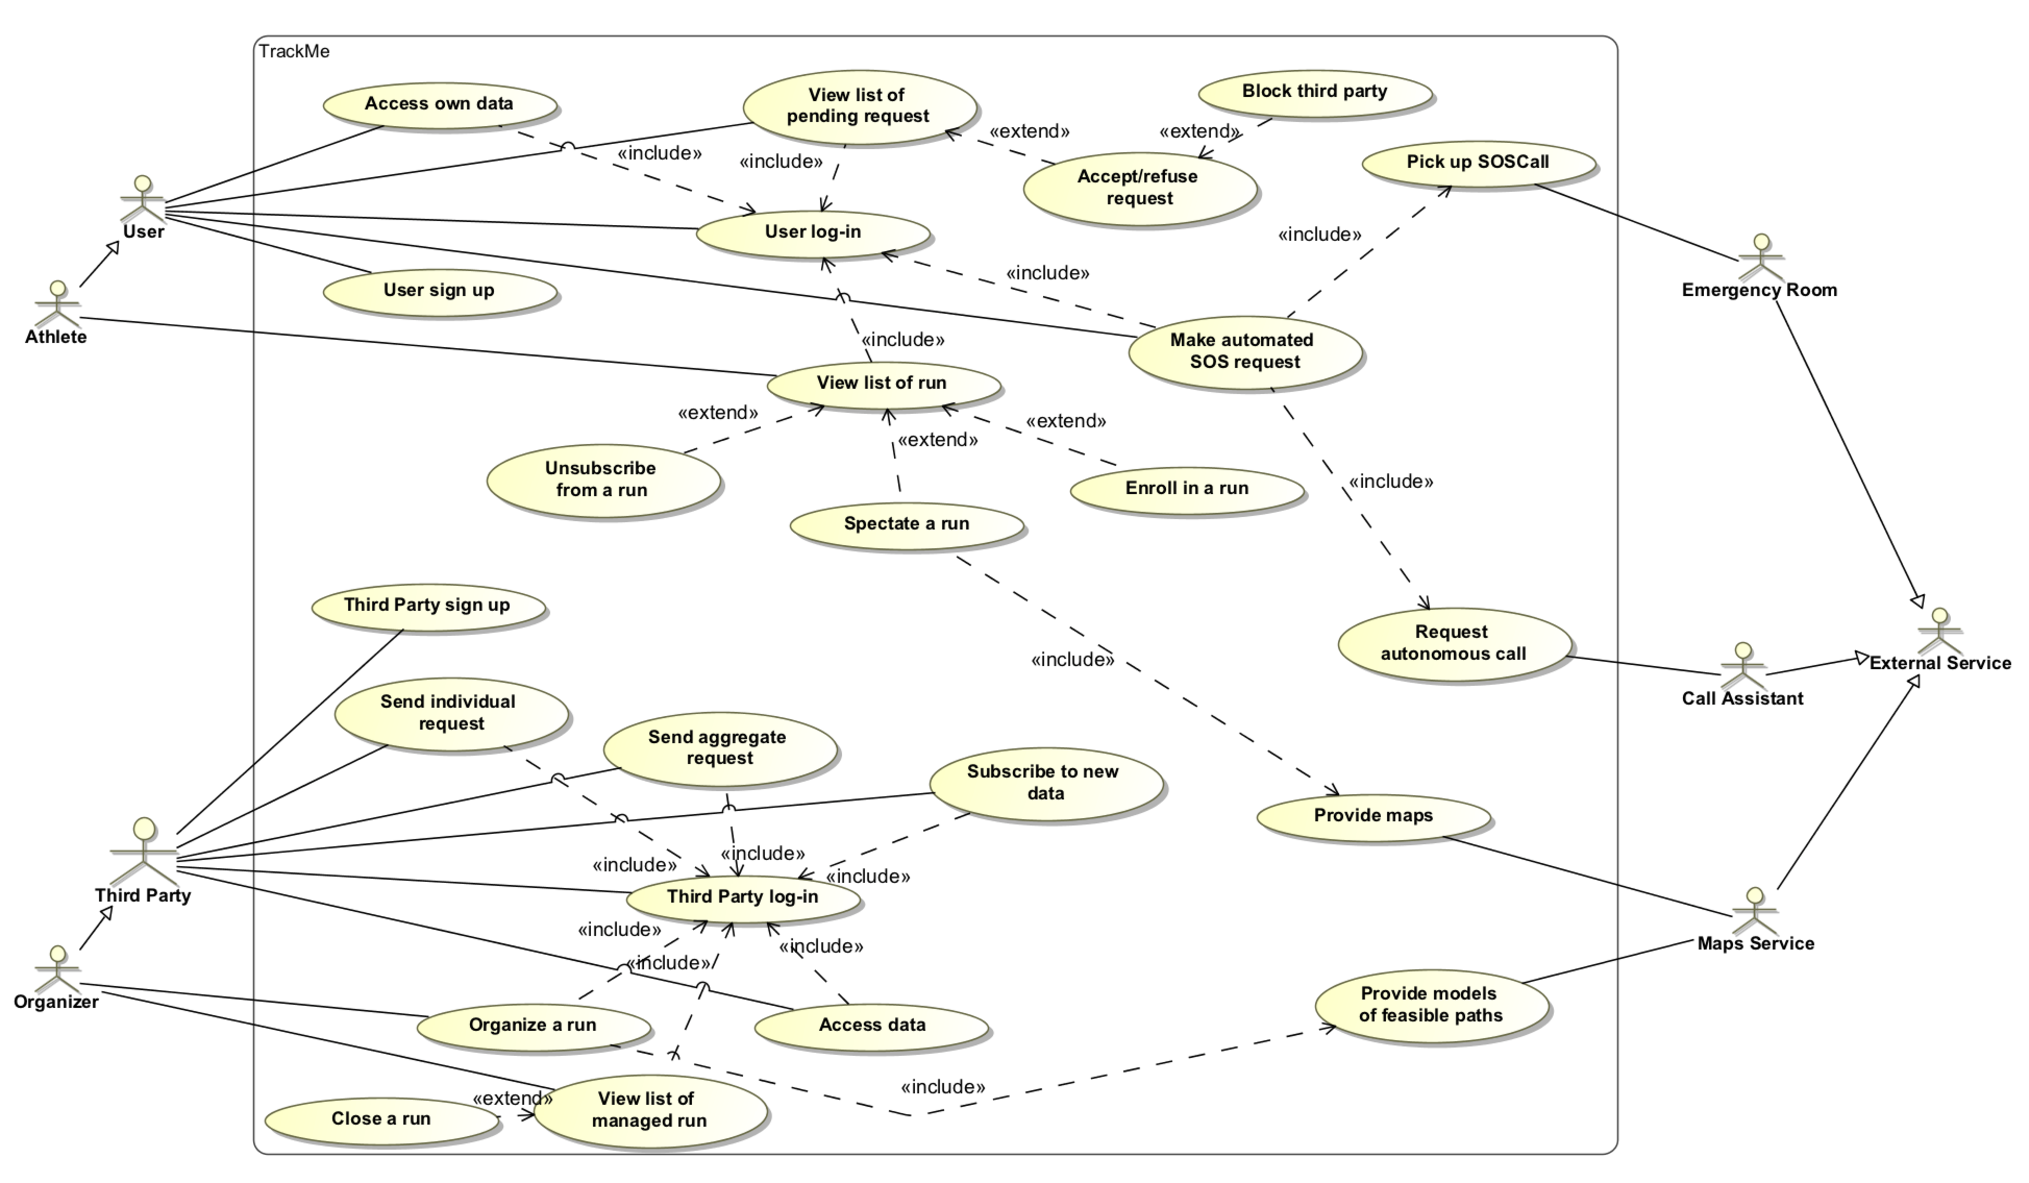
\includegraphics[width=\linewidth]{Images/usecase}
\caption{Use case diagram}
\label{fig:usecasediagram}
\end{figure}

\par 
Beneath, the use case are analyzed:	\\

\begin{table}[H]
\begin{tabularx}{\textwidth}{|l|X|}
\hline
 Name & Send aggregated request \\ \hline
 Actor & Third party customer  \\ \hline
 Entry conditions & Third party customer needs some aggregated data on anonymized users and the third party has performed log-in \\ \hline
 Event flow & 
 \begin{enumerate}
 	\item Third party customer compiles a form specifying the aggregated data that he wants to access
 	\item Third party customer sends the request
 	\item The system analyses the request and provides to the user the access to the data 
 \end{enumerate}   \\ \hline
 Exit conditions & The third party user can access the requested data \\ \hline
 Exceptions & If the request involves less or equal than 1000 distinct user, the access is not provided to the third party, that gets a notification \\ \hline
\end{tabularx}
\end{table}

\begin{table}[H]
\begin{tabularx}{\textwidth}{|l|X|}
\hline
 Name & Subscribe to new data \\ \hline
 Actor & Third party customer  \\ \hline
 Entry conditions & Third party customer needs some future aggregated data on anonymized users and the third party has performed log-in \\ \hline
 Event flow & 
 \begin{enumerate}
 	\item Third party customer compiles a form specifying the future aggregated data that he wants to access, when they will be available
 	\item Third party customer sends the request
 	\item The system waits for the moment in which all the future data requested will be generated 
 	\item The system analyses the request and provides to the user the access to the data 
 \end{enumerate}   \\ \hline
 Exit conditions & The third party user can access the requested data \\ \hline
 Exceptions & If the request involves less or equal than 1000 distinct user, the access is not provided to the third party, that gets a notification \\ \hline
\end{tabularx}
\end{table}

\begin{table}[H]
\begin{tabularx}{\textwidth}{|l|X|}
\hline
 Name & Organize run \\ \hline
 Actor & Third party customer \\ \hline
 Entry conditions & The third party customer has performed login and needs to organize a race\\ \hline
 Event flow & 
 \begin{enumerate}
 	\item The third party customer set up a run: he provides the name, the path, the date, the starting time, a closure date for the subscriptions and the minimum number of participants
  	\item The third party customer sends all the mentioned above information to the systme
 	\item The system adds the run to the list of the available races
 \end{enumerate}   \\ \hline
 Exit conditions & The race has been successfully added to the list of the available run \\ \hline
 Exceptions & 
 \begin{enumerate}
 	\item The name is already used by another run
 	\item Another run is already been specified for the same date and at least a portion of the path is overlapping 
 \end{enumerate}  
 All the exceptions are handled in the same way: the race is not added to the list and the third party user gets notified of the unsuccessful operation 
 \\ \hline
\end{tabularx}
\end{table}


\begin{table}[H]
\begin{tabularx}{\textwidth}{|l|X|}
\hline
 Name & Enroll in a run \\ \hline
 Actor & Athlete \\ \hline
 Entry conditions & The user wants to join to a run that has previously been added to the list of the available race \\ \hline
 Event flow & 
 \begin{enumerate}
 	\item The athlete accesses the list of available run
  	\item The athlete selects the race in which he wants to enroll
 	\item The athlete sends the request for joining the run to the system 
 	\item The system receives the requests and enroll the athlete in the race that he has specified 
 \end{enumerate}   \\ \hline
 Exit conditions & The athlete has been successfully enrolled to the race \\ \hline
 Exceptions &  
 \begin{enumerate}
 	\item The athlete is already enrolled to the race that he specifies in the request
 	\item The athlete is already been enrolled to a race in the same date of the run specified in the request 
 \end{enumerate}
 All the exceptions are handled in the same way: the athlete is notified that the enrollment was unsuccessful, by providing a brief motivation. Of course, the subscription process is aborted  
 \\ \hline
\end{tabularx}
\end{table}


\begin{table}[H]
\begin{tabularx}{\textwidth}{|l|X|}
\hline
 Name & Block requests from a company \\ \hline
 Actor & User \\ \hline
 Entry conditions & The user wants to block the request from a specific company \\ \hline
 Event flow & 
 \begin{enumerate}
 	\item The user accesses the list of available requests
  	\item The user selects the request which he wants to block
 	\item The user, with the express button, sends the request to TrackMe for classify as spam the selected request 
 	\item The system receives the requests and permanently blocks the company that sent the request.
 	\item The system notifies the user that the company is blocked
 \end{enumerate}   \\ \hline
 Exit conditions & The company had been successfully blocked \\ \hline
 Exceptions &  
 \begin{enumerate}
 	\item The company is already blocked.
 \end{enumerate}
 The exceptions are handled by the notification that the block of the company was unsuccessful, by providing a brief motivation.  
 \\ \hline
\end{tabularx}
\end{table}


\begin{table}[H]
\begin{tabularx}{\textwidth}{|l|X|}
\hline
 Name & Shared data with a third party\\ \hline
 Actor & User \\ \hline
 Entry conditions & The user wants to share data with a third party that it sent you a shared data request \\ \hline
 Event flow & 
 \begin{enumerate}
 	\item The user accesses the list of available requests
  	\item The user selects the request which he wants to accept
 	\item The user accept the request from a specific company
 	\item The system receives the acceptance and notifies both the third party and the user of the successful of the operation
 	\item The system provide the user health information to the third party
 \end{enumerate}   \\ \hline
 Exit conditions & The health status of the user is provided to the third party \\ \hline
 Exceptions &  
 \begin{enumerate}
 	\item The user accepts the request, but there are not available data in the system.
	\item The user accepts a request that has already accepted 
 \end{enumerate}
 The first exception is handle by notifying the third party that there are not available data stored in the system and it provides the data as soon as possible.
 The second exception is handle by notifying the user that the request has already accepted.
 \\ \hline
\end{tabularx}
\end{table}


\begin{table}[H]
\begin{tabularx}{\textwidth}{|l|X|}
\hline
 Name & Sign up \\ \hline
 Actor & User \\ \hline
 Entry conditions & The user wants to join to the application but he has not already registered \\ \hline
 Event flow & 
 \begin{enumerate}
 	\item The user click on the sign up button
  	\item The user complete the registration's form and provide his information
 	\item The user send the form to the system
 	\item The system checks that an account associated with identification information and social security number does not exists
 	\item The system notify to the user the success of the operation
 \end{enumerate}   \\ \hline
 Exit conditions & The user receive the notify about the successful of the operation \\ \hline
 Exceptions &  
 \begin{enumerate}
 	\item The user has already sign up into the application
 	\item The user doesn't provide valid data 
 	\item The username has already taken 
 \end{enumerate}
 The first exception is handle by notifying that the user has already subscribe into the application.
 All other exceptions are handled in the same way: the user is notified that the subscription was unsuccessful, by providing a brief motivation. The user is remanded to the sign up page.  
 \\ \hline
\end{tabularx}
\end{table}


\begin{table}[H]
\begin{tabularx}{\textwidth}{|l|X|}
\hline
 Name & Login \\ \hline
 Actor & User \\ \hline
 Entry conditions & The user wants to join into the application and he has already registered into the application\\ \hline
 Event flow & 
 \begin{enumerate}
 	\item The user enters his credentials in the “Username” and “Password” fields of the login page of “Data4Help” application 
  	\item The system checks the information provided by the user
 	\item The system redirects the user to the application home page
 \end{enumerate}   \\ \hline
 Exit conditions & The user is logged in the application \\ \hline
 Exceptions &  
 \begin{enumerate}
 	\item The user enters invalid username
 	\item The user enters invalid password 
 \end{enumerate}
 All the exceptions are handled in the same way: the user is notified that the logged in procedure was unsuccessful, by providing a brief motivation. Then the user is remanded to the login page.
 \\ \hline
\end{tabularx}
\end{table}

\subsubsection{Sequence diagrams}
To provide a better understanding of the interaction of some processes, the following diagrams are shown:
\begin{itemize}
\item Send individual request process
\begin{figure}[H]
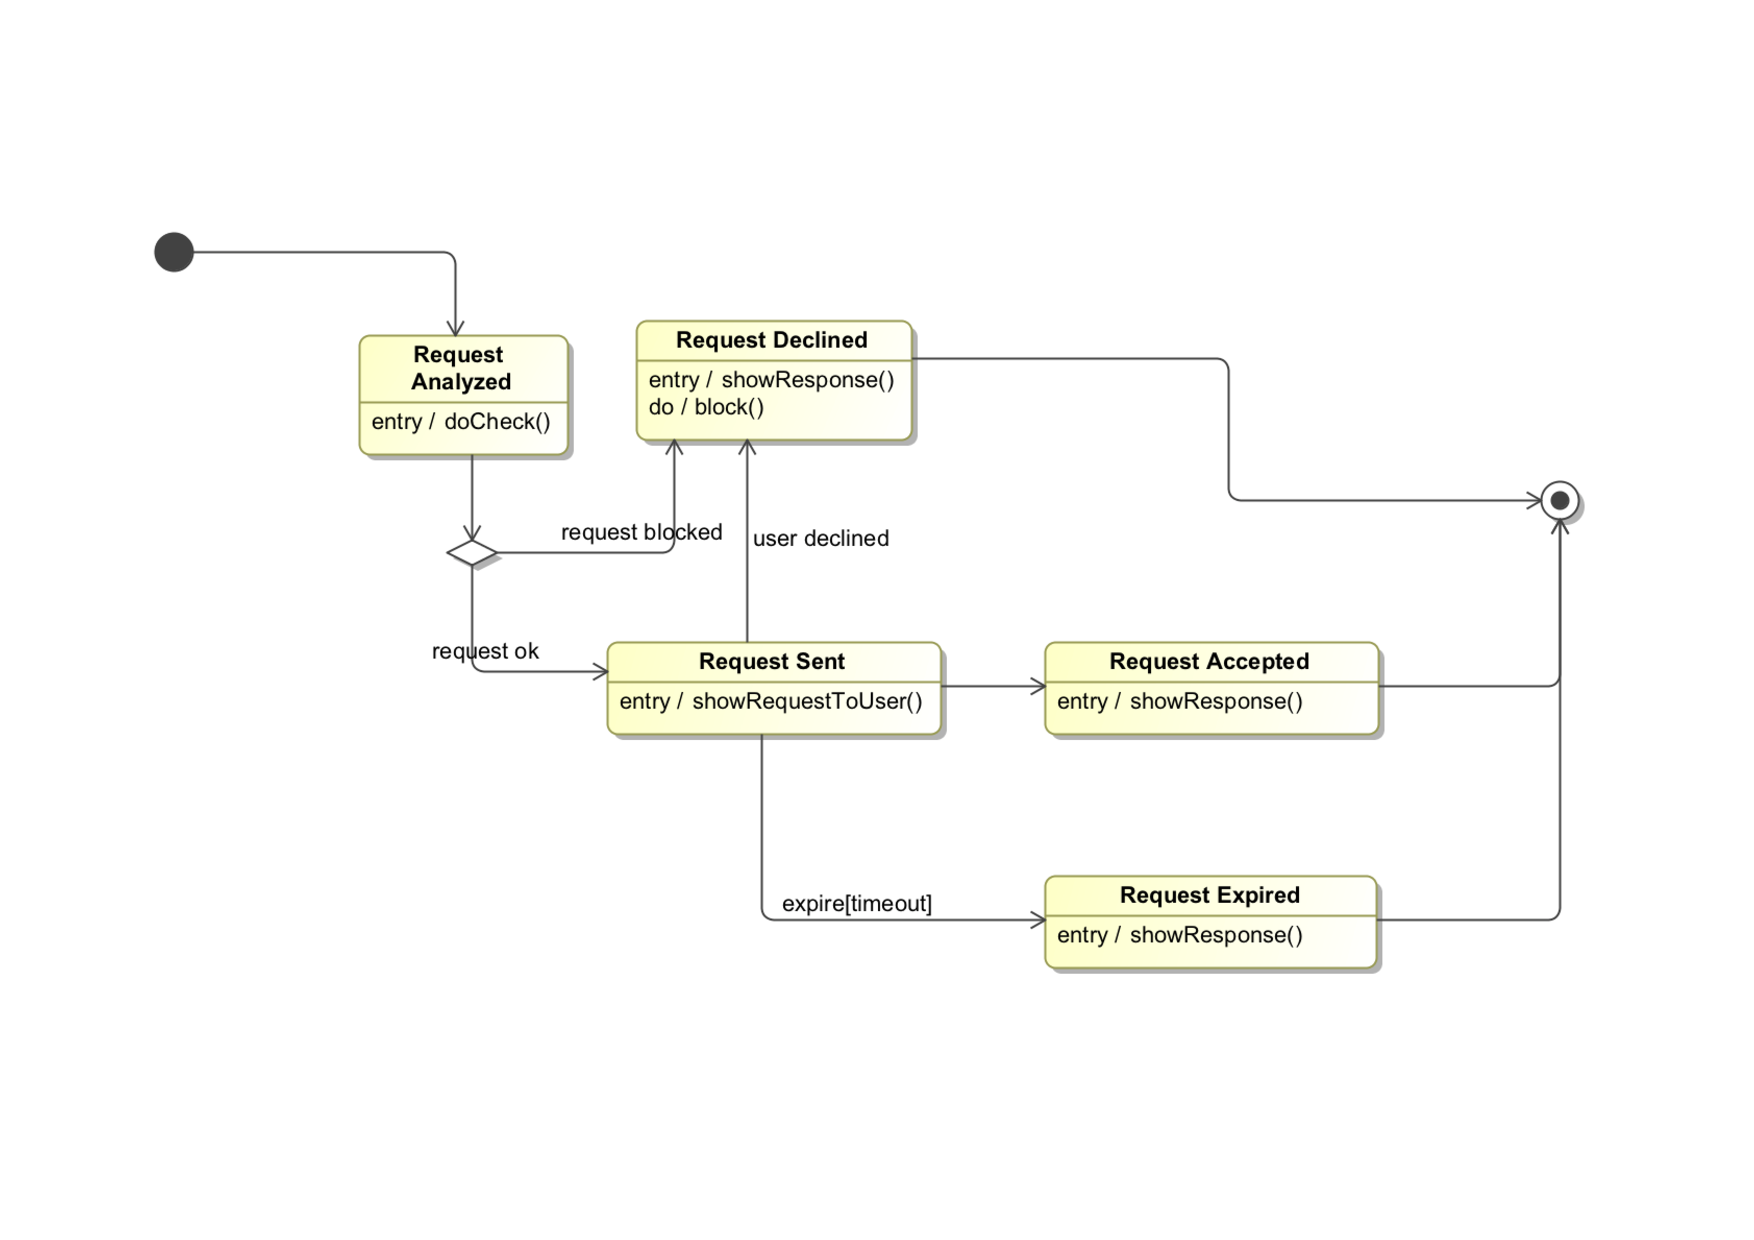
\includegraphics[width=\linewidth]{Images/requestdiagram}
\caption{Sequence diagram about the process of an individual request }
\label{fig:sequencediagram1}
\end{figure}

\item SOSCall process: the sequence diagram is designed by assuming that the process starts when for the first time the application has detected for the first time a health parameter below threshold.
\begin{figure}[H]
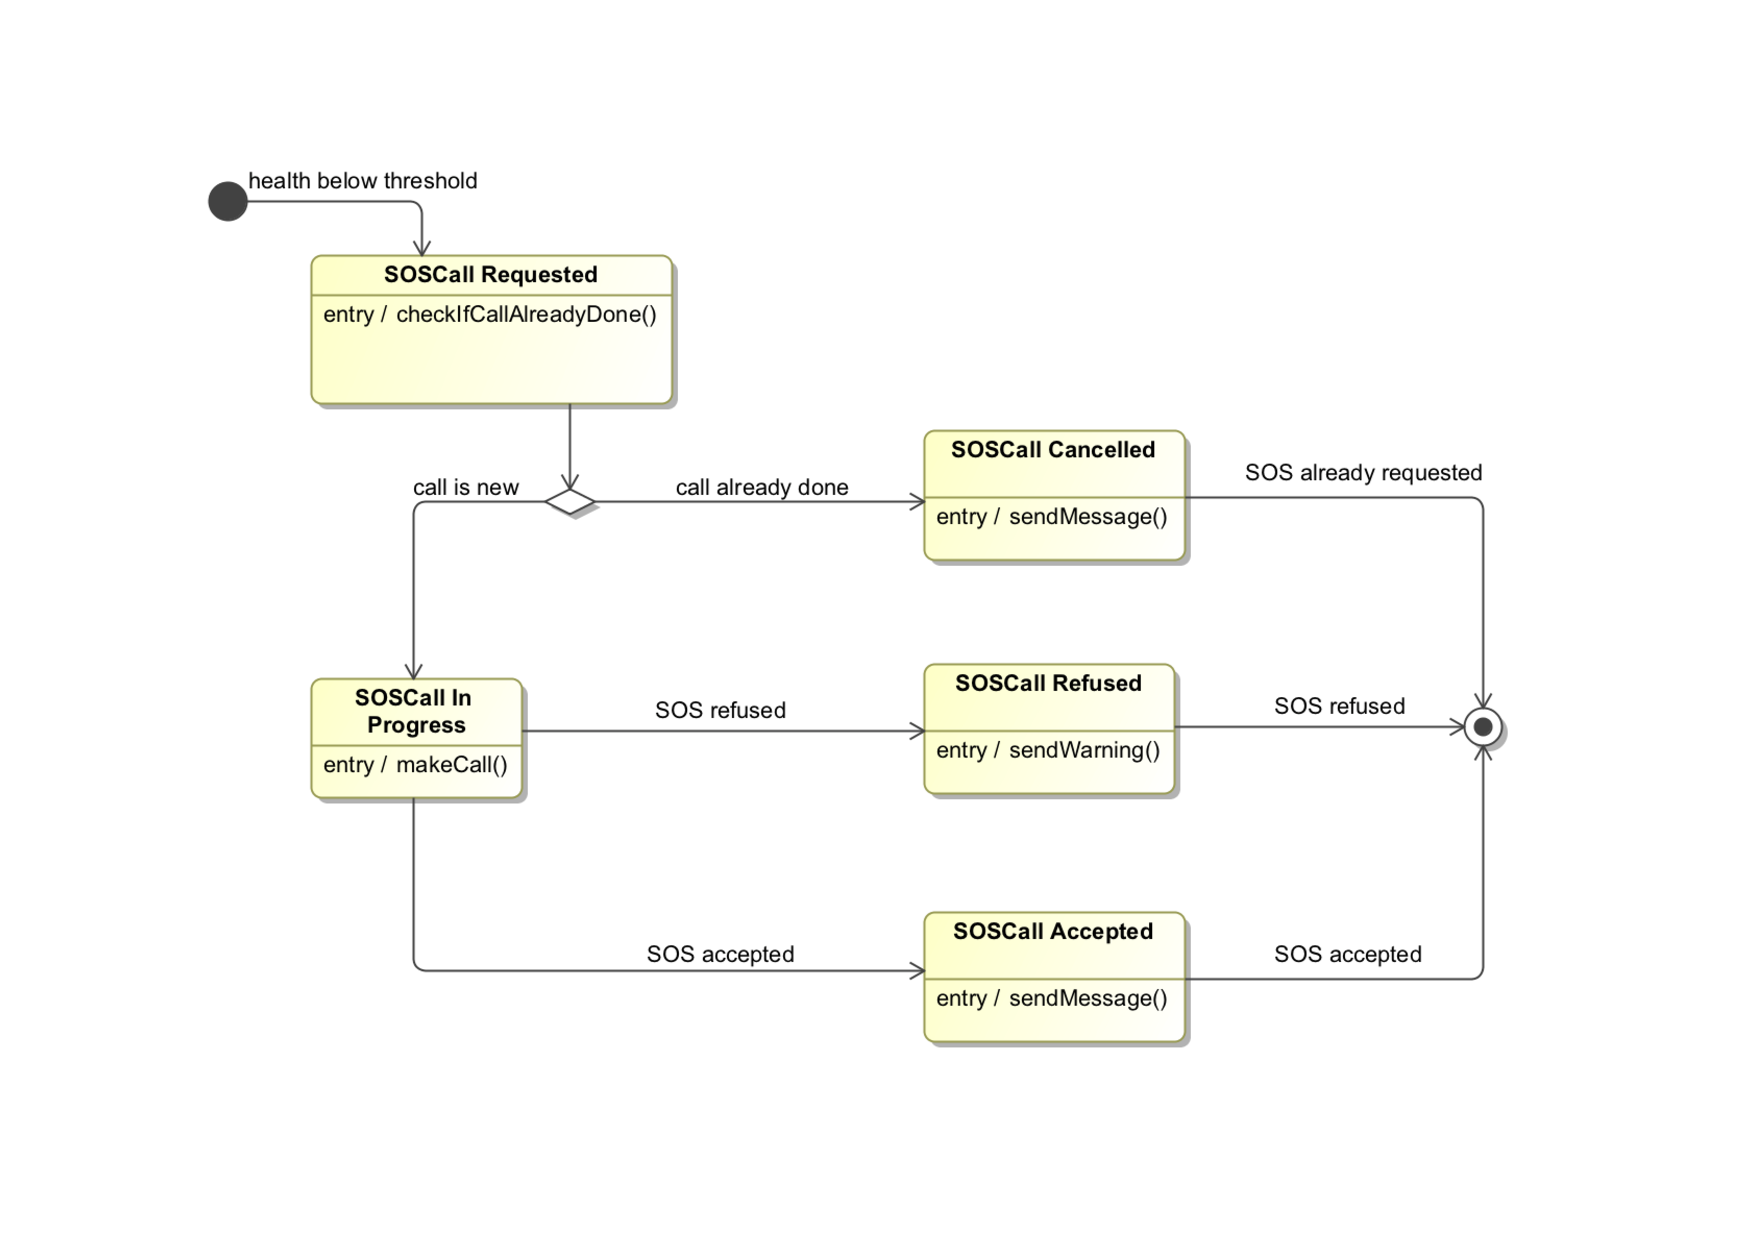
\includegraphics[width=\linewidth]{Images/sosdiagram}
\caption{Sequence diagram about the process of an SOS call }
\label{fig:sequencediagram2}
\end{figure}

\end{itemize}